In this section, the resiliency improvement due to automated attack generation is shown in simulation by implementing Algorithm~\ref{Alg:ADL_AAG_P} and the resilient Kalman filter of Theorem~\ref{Thm:resilient_estimation_gaurentee} on a water distribution system. The experiments also illustrate the sparsity--observability--precision--error bridge of Corollary~\ref{Cor:bridge}.

\begin{figure}[!ht]
    \centering
    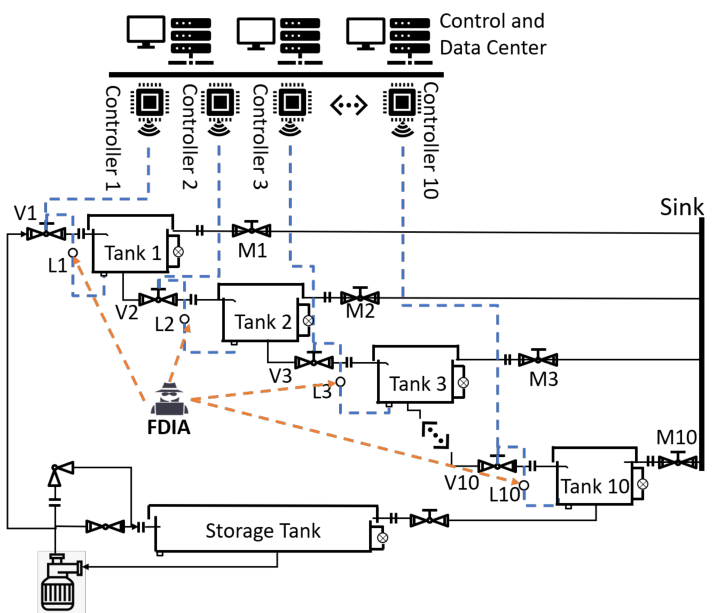
\includegraphics[width=\columnwidth]{image/WDS.png}
    \caption{Block diagram depiction of a water distribution system under \textcolor{blue}{FDIAs} (black solid are water pipelines, blue dotted lines are wireless data transmission lines for sensors data and control commands, orange dotted lines are attack injection route)}
    \label{fig:water_distribution_sys}
\end{figure}

The water distribution system, shown in Fig.~\ref{fig:water_distribution_sys}, contains $10$ distributed operating tanks and $1$ storage tank. The goal is to regulate all operating tanks' water levels around desired values. The magnetic valves $V_1 - V_{10}$ at the \textcolor{blue}{inlet} of operating tanks are controlled to adjust the water level of water tanks, and the manual valves $M_1 - M_{10}$ can be manipulated, at the demand point, to use the water from the corresponding tanks. The effect of these valves is modelled as the random demands $\mathbf{d}$ in \eqref{equ:water_level_adjustment}. The valves at the storage tank are fixed at a constant opening value.
\textcolor{blue}{For each operating tank, two sensors-water level meter and pressure sensors} ($L_1 ~ L_{10}$), are installed. The pressure sensors measure the difference of water level between adjoining tanks. The \textcolor{blue}{water levels} adjustment process is approximated by the LTI model:
\begin{equation}\label{equ:water_level_adjustment}
\begin{aligned}
   \mathbf{x}_{i+1} &= A\mathbf{x}_i + B\mathbf{u}_i - \mathbf{d}_i,\\
    \mathbf{y}_i &= C\mathbf{x}_i +\mathbf{v}_i + \mathbf{e}_i.
\end{aligned}
\end{equation}
where, $\mathbf{x}, \mathbf{u} \in \mathbb{R}^{10}$, \textcolor{blue}{$\mathbf{y}, \mathbf{v} \in \mathbb{R}^{61}$} are vector of water level, control input of magnetic valves, sensor measurements, and measurement noise respectively, $\mathbf{d} \in \mathbb{R}^{10}$ is the vector of random demands, and \textcolor{blue}{$\mathbf{e} \in \mathbb{R}^{61}$} is the injected \textcolor{blue}{FDIAs}. \textcolor{blue}{For the sake of clean presentation, interested readers are directed to \url{https://github.com/ZYblend/Resilient_WDS_AutoAttackGen} for the values of system parameters $A \in \mathbb{R}^{10\times 10},B \in \mathbb{R}^{10\times 10},C \in \mathbb{R}^{61\times 10}$.} Given \textcolor{blue}{a desired} water level $\mathbf{x}_d = 0.5 * \mathbf{1}_{10}$, \textcolor{blue}{the} proportional controller \textcolor{blue}{below} is used\textcolor{blue}{;}
$$ \mathbf{u}_i = -K(\hat{\mathbf{x}}-\mathbf{x}_d)-B^{-1}(A-I_{10})\mathbf{x}_d.
$$ 
The critical measurement in this scenario is the sum of all water levels of operating tanks, thus, the critical measurement matrix is given by $C_c = [1 \hspace{2mm} 1 \hspace{2mm} \cdots \hspace{2mm} 1] \in \mathbb{R}^{1\times 10}$. \textcolor{blue}{Firstly, a simulation experiment is done to assess the observability of the simulated system in order to obtain the least number of measurements from which the system states are fully observable. A Monte Carlos experiment, with $50000$ samples of randomly selected measurement subsets $\mathcal{S}$, is performed to calculated the probability of full observerability of $(A,C_{\mathcal{S}})$ using $|\mathcal{S}|$. Fig~\ref{fig:observability} shows that full observerability is preserved with $k_0 \geq 42$, corresponding to at most $30\%$ pruned measurements.}

\begin{figure}
    \centering
    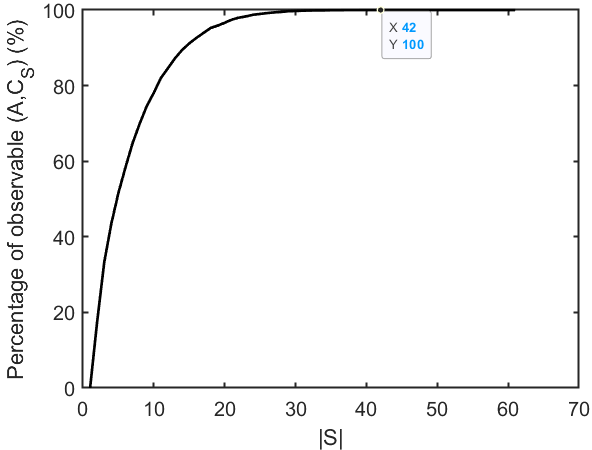
\includegraphics[scale=0.45]{new_sim_image/observability.png}
    \caption{\textcolor{blue}{Observability of simulated systems. The percentage of observable $(A,C_{\mathcal{S}})$ is calculated as the ratio of the number of observable $(A,C_{\mathcal{S}})$ to the total number of samples (=50000).}}
    \label{fig:observability}
\end{figure}

Next, we execute automated attack generation (against the KF/$\chi^2$ pair), MLP training, and Monte-Carlo simulation of the resilient KF under different detection/localization strategies.

\subsection{Automated attack generation}

A fixed time step of $T_s = 0.01s$ is used and the moving-window size is set as $T = 8T_s$. With different numbers of attacks, the discriminator maps $M_1$ (critical-output effectiveness through the KF--controller loop) and $M_2$ (chi-square stealthiness) are assembled for each random attack support. The generator in \eqref{equ:training_GM} is then trained as in Fig.~\ref{fig:GM}. Due to measurement noise and random demands, the thresholds are chosen as $\alpha = 0.1$ and $\epsilon=0.5$ (with $\epsilon$ aligned to the design chi-square level). Fig.~\ref{fig:train_result} shows effectiveness and the stealthiness statistic of generated attacks during training relative to $(\alpha, \epsilon)$. The trained generator maps uniform inputs to feasible attacks in \eqref{equ:success_FDIA_set}.
\begin{figure}[!h]
    \centering
    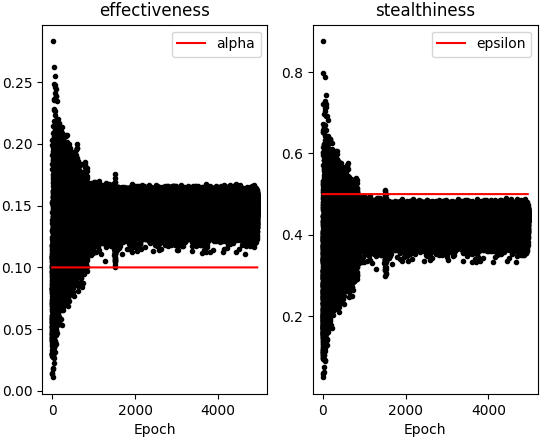
\includegraphics[scale=0.6]{new_sim_image/training_result.png}
    \caption{Feasibility of generated attacks during training. $\epsilon$ upper-bounds the chi-square stealthiness statistic $\|M_2 e\|_2$; $\alpha$ lower-bounds KF--controller effectiveness $\|M_1 e\|_2$.}
    \label{fig:train_result}
\end{figure}

\textcolor{blue}{The trained generator is then used to generate a dataset $D_\mathcal{S}(\alpha,\epsilon)$ of attacks. In order to inject the generated attacks, recursive feasibility \cite{lofberg2012oops} should be considered. An online moving-horizon attack injection scheme used here is to solve the following sample-based optimization program at each time step $i$: 
\begin{equation} \label{equ:attack_injection}
\begin{aligned}
       \displaystyle\Maximize_{\mathbf{e}_i} \hspace{2mm} &\left\|M_1 \begin{bmatrix}\mathbf{e}^{-} \\ \mathbf{e}_i\end{bmatrix}\right\|_2 \\
    \textsf{Subject to:} \hspace{2mm} & \left\|M_2 \begin{bmatrix}\mathbf{e}^{-} \\ \mathbf{e}_i\end{bmatrix}\right\|_2 \leq \epsilon \\
    & \mathbf{e}_i \in D_\mathcal{S}(\alpha,\epsilon)
\end{aligned}
\end{equation}
where $\mathbf{e}^{-}$ is the attack history during the time window $I^{-} = [i-T+1, i-1]$. Fig.~\ref{fig:generator_test_example_1} shows the performance of the generated attacks under the injection program \eqref{equ:attack_injection}.} The left panel shows that the windowed chi-square / innovation statistic under attack stays close to the nominal (attack-free) trajectory, i.e., the attacks remain stealthy relative to \eqref{equ:chisq_detector}. The right panel shows a clear deviation of the critical measurement, confirming effectiveness through the KF--controller loop.
\begin{figure}[!h]
    \centering
    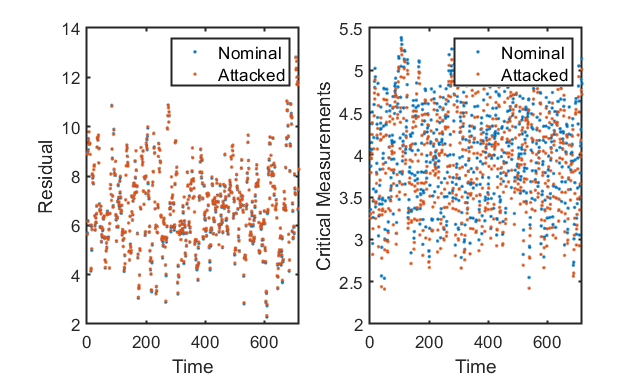
\includegraphics[width=\columnwidth]{new_sim_image/attack_effect.png}
    \caption{Performance of generated attacks injected through $39\%$ measurement nodes. (Left: windowed innovation / chi-square stealthiness statistic; Right: critical measurement.)}
    \label{fig:generator_test_example_1}
\end{figure}

 \textcolor{blue}{Next, the above automated attack generation scheme is trained to generate different types of attacks including different attack supports and different number of attacks. The generated attacks are then used to train the supervised learning-based attack detection and localization algorithm in next subsection.}

\subsection{MLP training}
To show one of the merits of the proposed automated attack generation scheme, two training datasets are prepared: one produced by random additive signals on measurements and the other augments the dataset with attack samples generated by the trained generator. Next, two MLP classifiers are trained on two datasets respectively. \textcolor{blue}{MLP1 and MLP2 are both four-layer fully-connected neural network with three "relu" hidden layers of $512, 1024, 512$ neurons respectively.  The output layer has $61$ neurons and uses "sigmoid" activation function. MLP1 is trained by the first random attack dataset, while MLP2 is trained the second training dataset containing automated generated attacks. The testing F1 score and precision of MLP1 are $85.1\%$ and $99.7\%$ respectively, while MLP2 achieves $88.7\%$ and $99.1\%$ respectively. The testing datasets used is $10\%$ of the corresponding datasets, so the testing datasets for MLP2 and MLP1 are different. Next, we compare the localization precision of the two MLPs on a same testing dataset which is an equal mixture of dataset 1 and dataset 2. As shown in Fig.~\ref{fig:MLP_compare}, MLP2 has successfully shifted the localization precision to the right, indicating a better performance overall. However, MLP1's performance is nearly uniform for different localization precision higher than $0.5$. This is because it is trained by random attack dataset. The mean precision of MLP1 is $74.37\%$, and the mean precision of MLP2 is $98.69\%$ on a testing set of successful \textcolor{blue}{FDIAs}.}   

\begin{figure}[!ht]
    \centering
    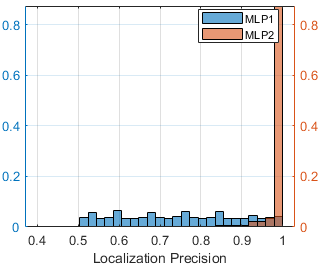
\includegraphics[scale=0.8]{new_sim_image/MLP_compare.png}
    \caption{\textcolor{blue}{A sample-based comparison of the performance of two MLP classifiers on same testing set of successful FDIAs. (MLP1: trained only with random attack generation, MLP2: trained with random attack generation and the proposed automated attack generation, $50000$ test cases are used.)}}
    \label{fig:MLP_compare}
\end{figure}

\begin{figure}[!ht]
    \centering
    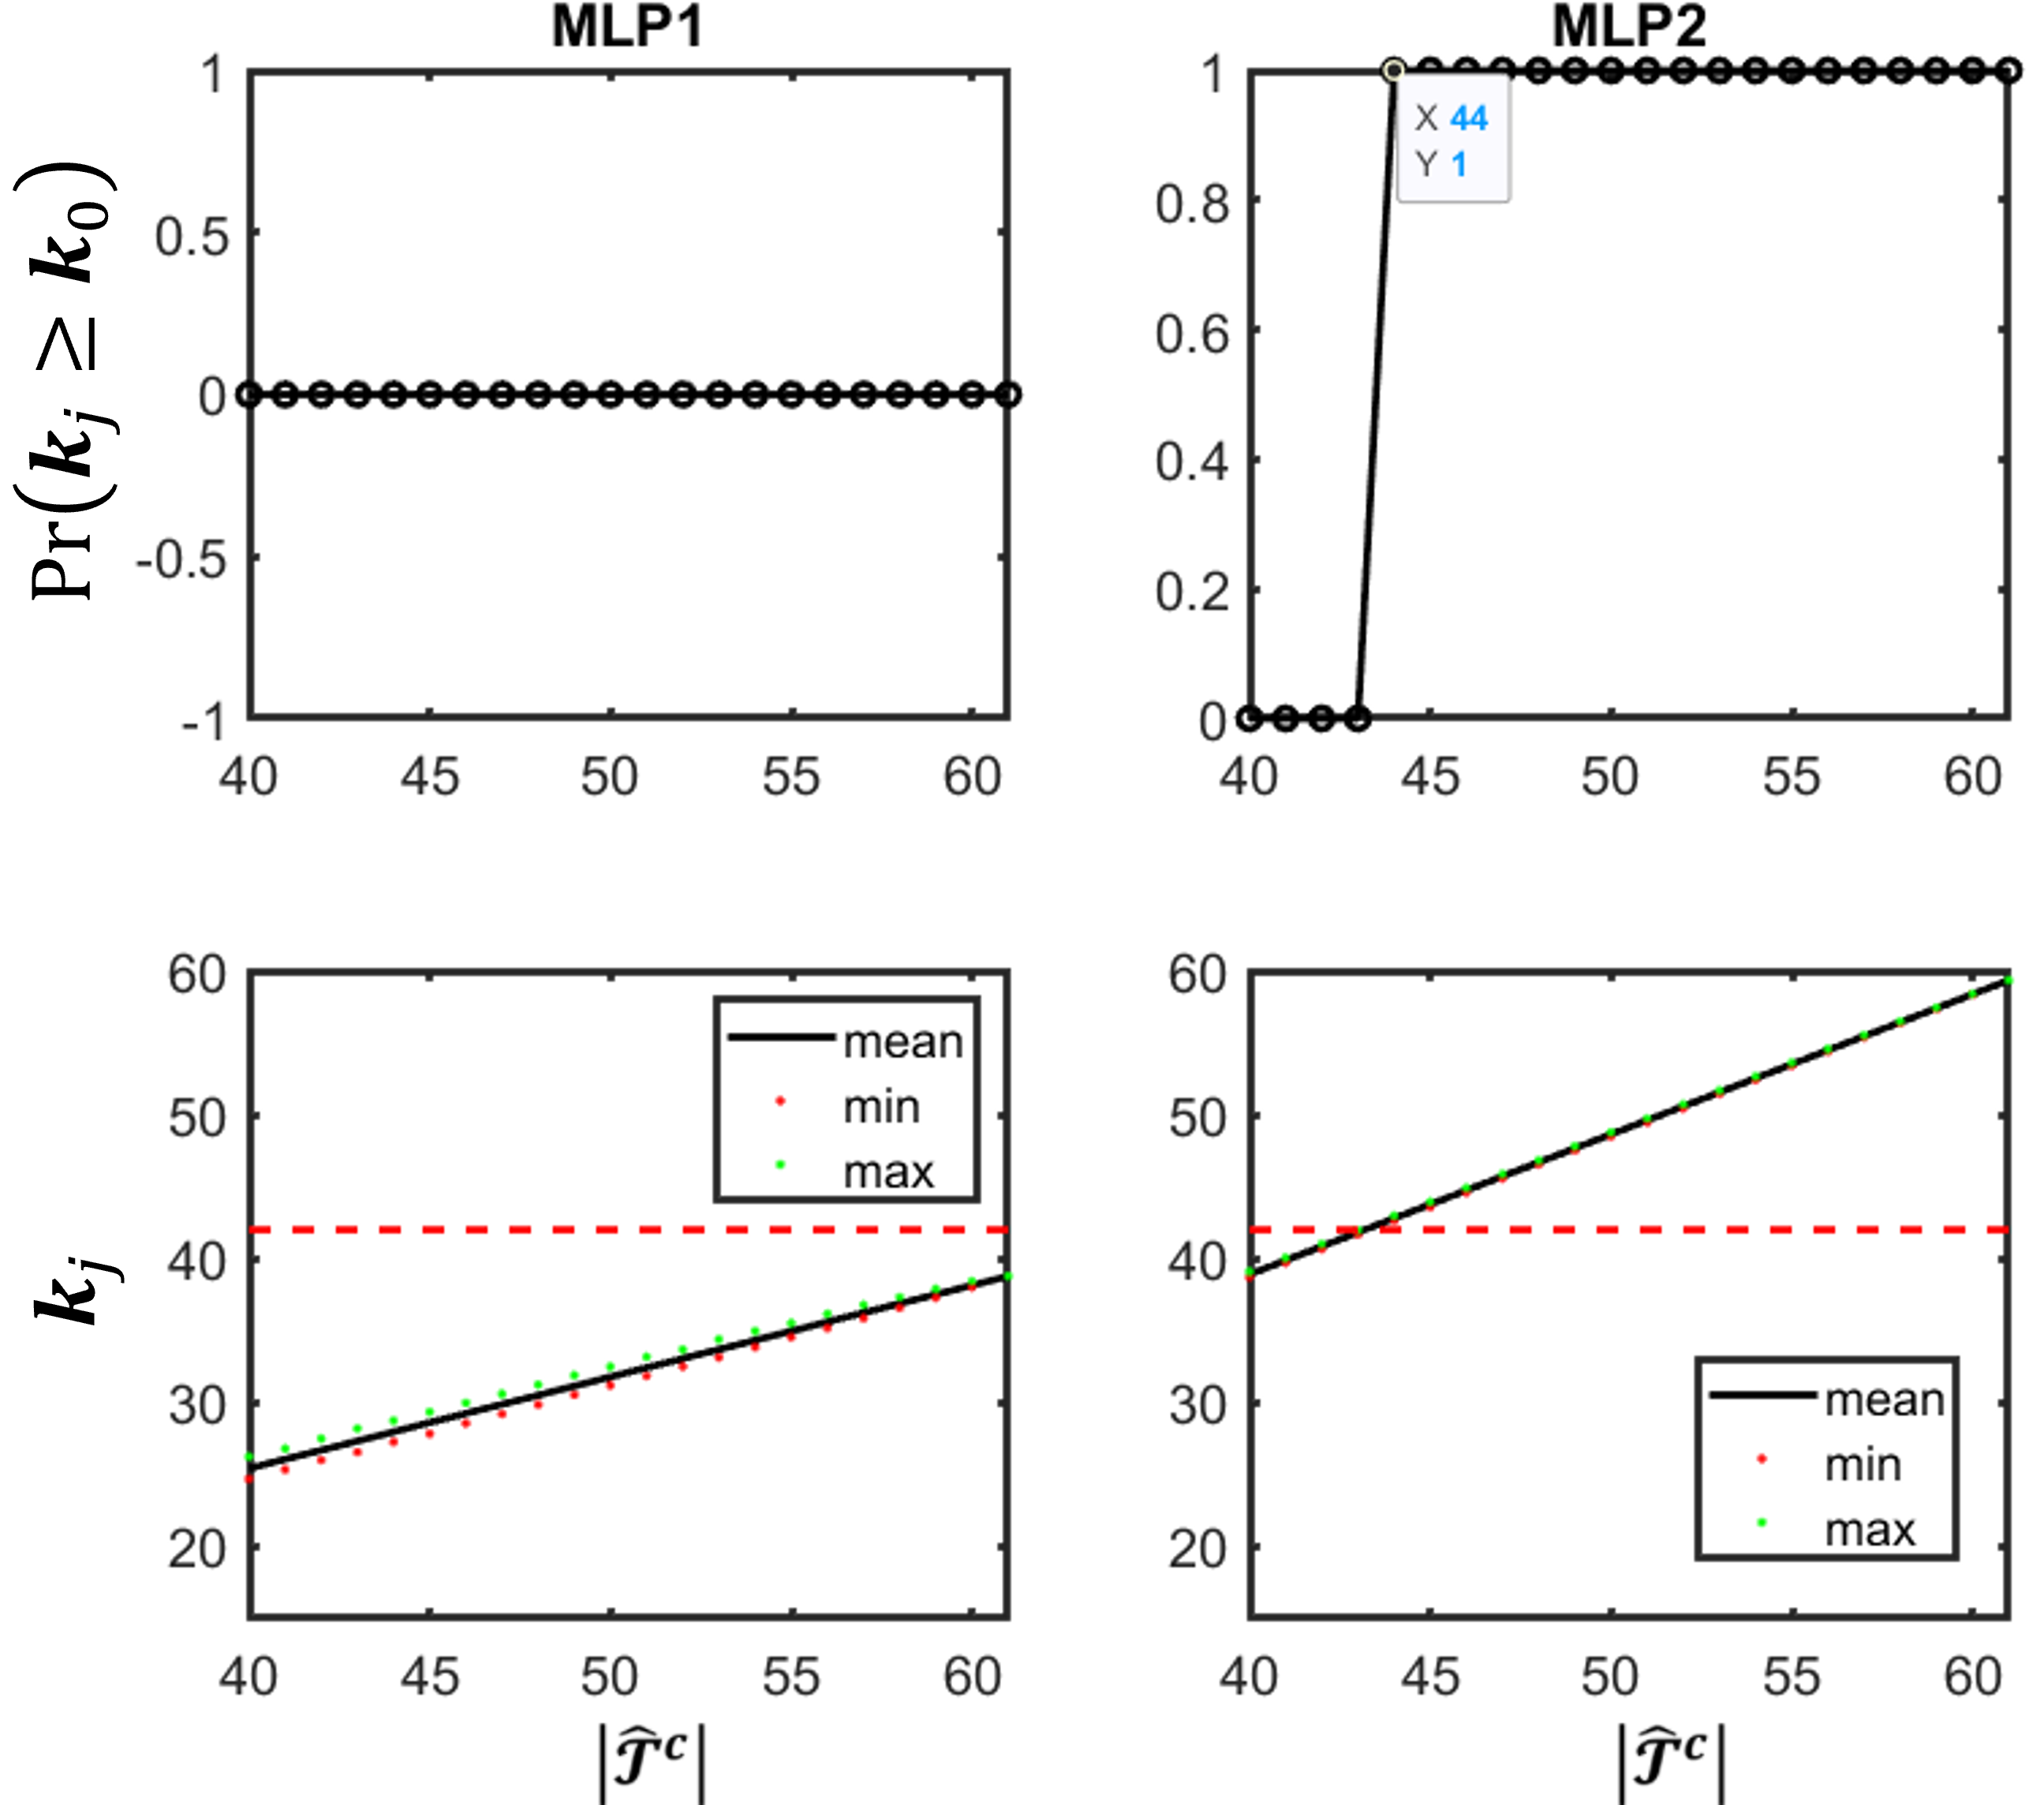
\includegraphics[scale=0.4]{new_sim_image/post_pruning_observability.png}
    \caption{\textcolor{blue}{A sample-based comparison of post-pruning observability for MLP1 and MLP2. ($50000$ test cases are used. The y axis for the top two subplots $Pr(k_j\geq k_0)$ is the sample estimate of the probability of at least $k_0$ measurements remaining after pruning. The black lines in the bottom subplots show the mean value of $k_j$ that is the number of measurements remaining after pruning, while the red and green dots are the minimum and maximum values of $k_j$'s respectively.}}
    \label{fig:MLP_compare_k0}
\end{figure}

As shown in Fig.~\ref{fig:observability}, full observability can be guaranteed with certainty if \textcolor{blue}{$k_0\geq 42$} measurements remains after pruning. For this, we evaluate the sufficient condition in \eqref{equ:localization_performance_criterion} on MLP1 and MLP2. First, the two MLPs are run on $10000$ cases generated by the trained generative model. From the results, the confidence vectors of the MLPs are estimated by calculating the true rates at all $61$ measurement nodes; for node $i$, $\mathbf{p}_i=\frac{TP_i+TN_i}{P_i+N_i}$. 
\iffalse
The confidence vectors of MLP1 and MLP2 are
$$\begin{aligned}
   &\mathbf{p}(\text{MLP1}) = [0.7076, 0.7065, 0.6883, 0.6621, 0.6855, 0.6790,\\
   &0.6721, 0.6807, 0.6623, 0.6791, 0.7535, 0.7610, 0.7519, 0.7334, \\
   &0.7692, 0.8001, 0.7393, 0.7150, 0.7667, 0.7519, 0.7544, 0.7338, \\
   & 0.7402, 0.7362, 0.7759, 0.7418, 0.7474, 0.7382, 0.7476, 0.7831, \\
   &0.7446, 0.7645, 0.7742, 0.7378, 0.7938, 0.7652, 0.7635, 0.7771, \\
   &0.7633, 0.7646],
\end{aligned} 
$$
$$\begin{aligned} &\mathbf{p}(\text{MLP21}) = [0.9826, 0.9819, 0.9828, 0.9853, 0.9866, 0.9737,\\
   &0.9804, 0.9858, 0.9748, 0.9749, 0.7692, 0.7685, 0.7764, 0.7855, \\
   &0.7667, 0.7995, 0.7422, 0.7528, 0.7729, 0.7959, 0.7631, 0.7996, \\
   & 0.7870, 0.7581, 0.7899, 0.7533, 0.7801, 0.8237, 0.7883, 0.8227, \\
   &0.7664, 0.7772, 0.8087, 0.8039, 0.8226, 0.8470, 0.8157, 0.8443, \\
   &0.8044, 0.8257].
\end{aligned} $$
\fi
Next, a sample based experiment is performed. For each support size \textcolor{blue}{$|\hat{\mathcal{T}}_j^c| \in \left\{40,41,\hdots,61\right\}$}, we generated  $\min\left\{^{61}C_{|\hat{\mathcal{T}}_j^c|},50000\right\}$ unique supports $\hat{\mathcal{T}}^c$, and  evaluated the right hand side of \eqref{equ:localization_performance_criterion} for each unique support as follows: 
$$k_j = -\ln\left(\sum_{i=0}^{|\hat{\mathcal{T}}_j^c|}e^{-i}\bar{\mathbf{r}}_i\right),$$
where the Poisson-binomial probability density vector $\bar{\mathbf{r}}_i$ is calculated, using the confidence vectors of \textcolor{blue}{the corresponding MLP}, based on \eqref{equ:r_tau_hat_c}. For each \textcolor{blue}{$|\hat{\mathcal{T}}_j^c| \in \left\{40,41,\hdots,61\right\}$}, and each MLP, the sample probability of the event $k_j\ge k_0$ and the expected value of $k_j$ are shown in Fig.~\ref{fig:MLP_compare_k0}. The results show that  MLP2 has a bigger chance of preserving post-pruning observability. Indeed, according to the figure, post-pruning observability cannot be guaranteed when MLP1 is used. \textcolor{blue}{In addition, from the bottom plots in Fig.~\ref{fig:MLP_compare_k0}, it is seen that MLP2 reduces the uncertainty on the post-pruning observability compared to MLP1.} By considering the sample-based analysis in Fig.~\ref{fig:MLP_compare} and Fig.~\ref{fig:MLP_compare_k0} together, it is seen that MLP performs better \textcolor{blue}{when trained with data generated by} the proposed automated attack generation.

Next, we compare MLP1 and MLP2 inside the resilient KF scheme.

\subsection{Resilient Kalman filter}
The trained MLPs, with and without pruning, are embedded in the real-time WDS simulation with the resilient KF of Section~\ref{sec:resilient_estimator}. A Monte-Carlo experiment estimates: (1)~the \textbf{probability of sustaining normal operation} (pSNO)---the fraction of times the critical-measurement deviation stays below a threshold; (2)~the \textbf{probability of triggering an alarm} (pTA)---the fraction of times the chi-square / innovation statistic exceeds its attack-free baseline by a threshold. Larger pSNO and pTA indicate better resiliency.

Attacks with sparsity from $1$ to $30$ are considered (five random-support scenarios each). For each detector variant (MLP1, MLP1+pruning, MLP2, MLP2+pruning), the pipeline in Fig.~\ref{fig:resilient_L2_observer} is simulated. Let $g_I$ denote the windowed chi-square statistic and $\mathbf{y}_{c_{i+1}}$ the critical output. Normalized deviations
$$\begin{aligned}
    \Delta g &= \frac{\left|(g_{I}-g_d)-(g^{\star}_{I} - g_d)\right|}{\textsf{max}\left(\left|(g_{I}-g_d)-(g^{\star}_{I} - g_d)\right|\right)}, \\
\Delta \mathbf{y} &= \frac{\left|(\mathbf{y}_{c_{i+1}}-\mathbf{y}_{c_d})-(\mathbf{y}^{\star}_{c_{i+1}}-\mathbf{y}_{c_d})\right|}{\textsf{max}\left(\left|(\mathbf{y}_{c_{i+1}}-\mathbf{y}_{c_d})-(\mathbf{y}^{\star}_{c_{i+1}}-\mathbf{y}_{c_d})\right|\right)},
\end{aligned}
$$
are formed relative to the attack-free noise-free baselines $g_d$ and $\mathbf{y}_{c_d}=C_c\mathbf{x}_d$. Then
$\mathrm{pTA}=\tfrac{1}{N}\|\Delta g \ge \tau_1\|_{\ell_0}$ and
$\mathrm{pSNO}=\tfrac{1}{N}\|\Delta \mathbf{y}\le \tau_2\|_{\ell_0}$,
with $\tau_1=1\%$ and $\tau_2=3\%$ calibrated on attack-free runs. These metrics empirically probe Corollary~\ref{Cor:bridge}: as sparsity $k$ grows, preserving $|\hat{\mathcal{T}}^c_{\eta}|\ge k_0=42$ and high $\textsf{PPV}_{\eta}$ becomes harder, which appears as degraded pSNO/pTA unless localization (MLP2) is strong enough.

\begin{figure}[!ht]
    \centering
    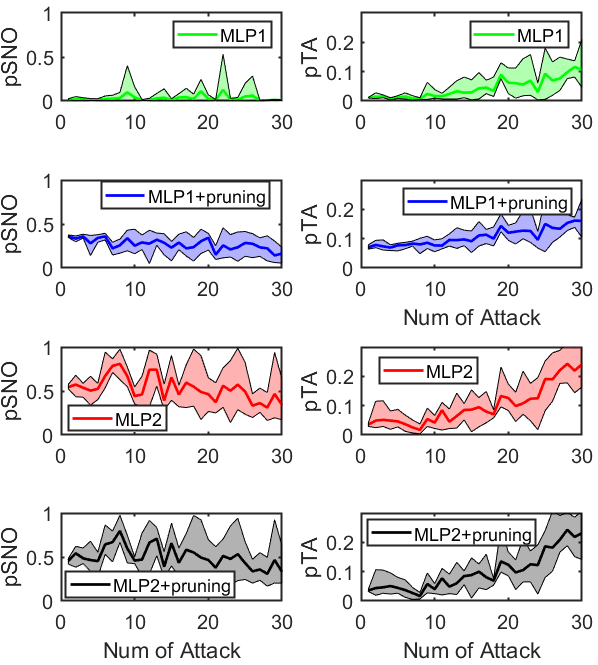
\includegraphics[scale=0.5]{new_sim_image/resiliency_compare.png}
    \caption{Resilient KF performance under different attack detection strategies; larger pSNO and pTA indicate better resiliency. Solid lines are means; shaded regions indicate spread.}
    \label{fig:resiliency_compare}
\end{figure}

Fig.~\ref{fig:resiliency_compare} compares pSNO and pTA across strategies. MLP2 outperforms MLP1 (and even MLP1+pruning), showing the value of generator-augmented training. Mean localization precision \eqref{equ:PPV_def} versus number of attacks is shown in Fig.~\ref{fig:precision}. Pruning still raises MLP2 precision, but state-estimation gains saturate once the observability budget $k_0$ binds---consistent with the $\eta$--$l_{\eta}$--$\mathrm{tr}\,P_{\infty}$ trade-off in Proposition~\ref{Prop:precision_observability} and Theorem~\ref{Thm:resilient_estimation_gaurentee}. MLP2+pruning nevertheless tightens the spread of pSNO/pTA, i.e., reduces performance uncertainty.


\begin{figure}[!ht]
    \centering
    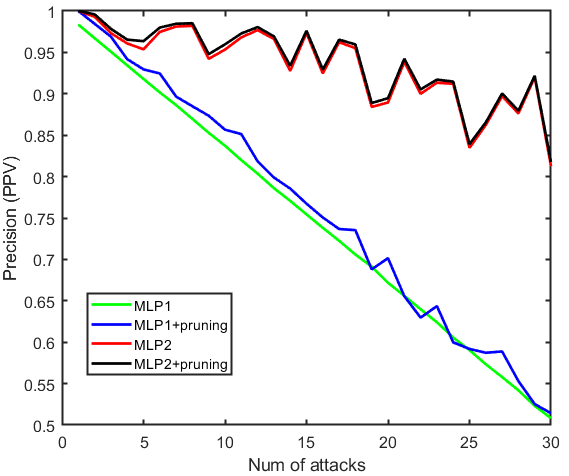
\includegraphics[scale=0.5]{new_sim_image/precision_vs_num_attack.png}
    \caption{\textcolor{blue}{A comparison of the mean precision of different attack detection strategies in the system simulation versus different number of attacks}}
    \label{fig:precision}
\end{figure}

\iffalse
\begin{table}[]
    \centering
    \caption{Mean value of attack localization precision}
    \begin{tabular}{|c|c|c|c|c|}
    \hline
       $\#$(attacks) & MLP1 & MLP1+pruning & MLP2 & MLP2+pruning  \\
        \hline 
       2  &  0.9150 & 0.9696 & 0.9559 & 0.9993\\
       3 & 0.8853 & 0.9427 & 0.9282 & 0.9790\\
       4 & 0.8612 & 0.9182 & 0.8998 & 0.9536\\
       5 & 0.8356 & 0.8925 & 0.8778 & 0.9381 \\
       6 & 0.8148 & 0.8651 & 0.8645 & 0.9201 \\
       7 & 0.7903 & 0.8414 & 0.8402 & 0.8878 \\
       8 & 0.7672 & 0.8116 & 0.8234 & 0.8823 \\
       9 & 0.7434 & 0.7905 & 0.7993 & 0.8677 \\
       10 & 0.7150 & 0.7602 & 0.7719 & 0.8407 \\
       11 & 0.6905 & 0.7377 & 0.7501 & 0.8296 \\
       12 & 0.6651 & 0.7091 & 0.7174 & 0.7904 \\
       13 & 0.6441 & 0.6851 & 0.7011 & 0.7689 \\
       14 & 0.6167 & 0.6598 & 0.6705 & 0.7496 \\
       15 & 0.5704 & 0.6349 & 0.6517 & 0.7388\\
       16 & 0.5704 & 0.6106 & 0.6412 & 0.7223\\
       17 & 0.5462 & 0.5833 & 0.6135 & 0.6955 \\
       18 & 0.5251 & 0.5576 & 0.5983 & 0.6751 \\
       19 & 0.5012 & 0.5305 & 0.5641 & 0.6265 \\
       20 & 0.4725 & 05069 & 0.5296 & 0.6192\\
       \hline
    \end{tabular}
    \label{tab:precision_table}
\end{table}
\fi


Finally, Fig.~\ref{fig:time_domain_result} shows a time-domain comparison under the same $39\%$ compromised measurements as in Fig.~\ref{fig:generator_test_example_1}. Schemes using MLP2 (with or without pruning) reduce critical-output deviation (smaller $\Delta \mathbf{y}$) while increasing the chi-square / innovation excursion (larger $\Delta g$), i.e., attacks become both less effective and less stealthy once the resilient KF is fed a high-precision safe set.

\begin{figure}[!ht]
    \centering
    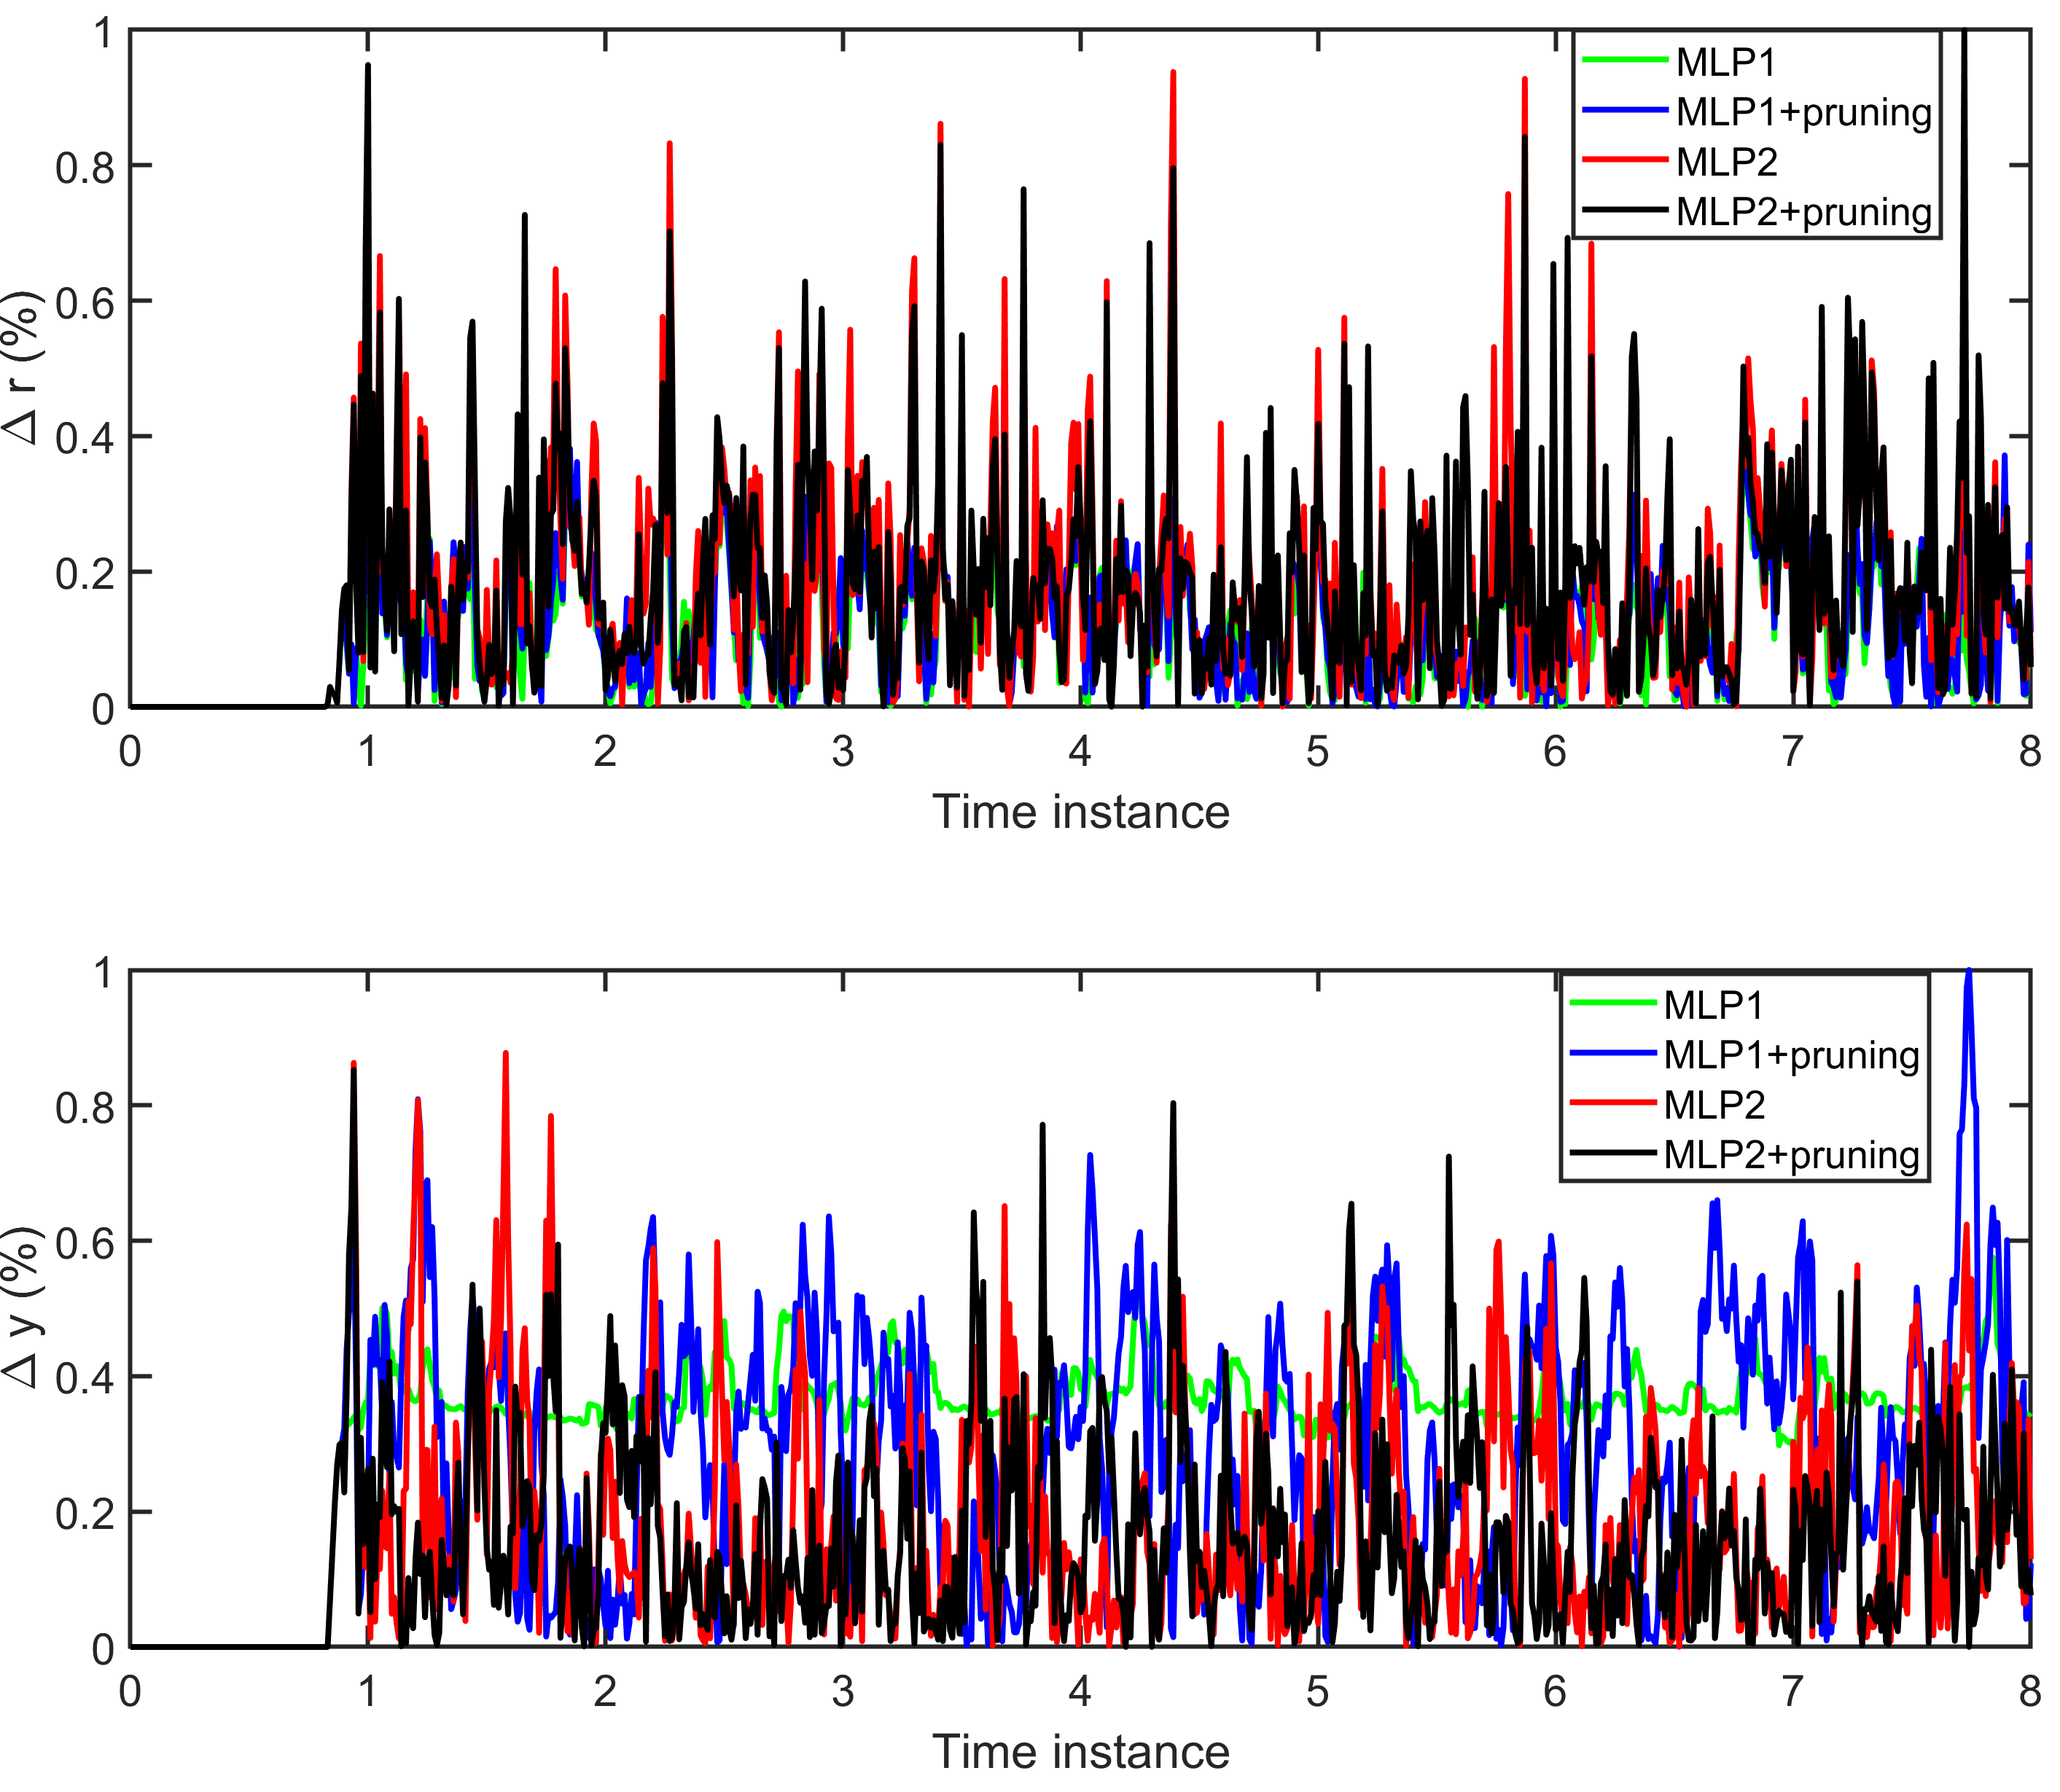
\includegraphics[scale=0.11]{new_sim_image/time-domain.png}
    \caption{Time-domain resilient KF results for four localization strategies under the attack scenario of Fig.~\ref{fig:generator_test_example_1}.}
    \label{fig:time_domain_result}
\end{figure}
